% !TEX root = ../main.tex
\section{Results and Evaluation}\label{sec:results-and-evaluation}
In this section, we will discuss the results that we were able to achieve from the project. Explanations will be given for successes and failures, with theories for why results may not have been as expected.

% State specification and how each was met
% What works well? What doesn't work well? (reliable, performant, response times, robust)
% Evaluation by potential users

\subsection{Landing Pattern Generation}
The landing pattern generation feature was a `Must' in the requirements for this project. Another requirement was that the landing patterns generated must be for a customisable target landing area and current wind conditions.
The project has succeeded in fulfilling both landing pattern generation requirements, offering an easy to use and intuitive interface.
When comparing generated landing patterns from the app with expected landing patterns identified by a skydiver, they were either the same or very similar. Variations came from estimations of canopy travel distance from the skydiver as well as inaccurate wind data.

Confirmation that the app produces sensible landing patterns can be seen in Figure~\vref{fig:predicted-tracked} where a landing pattern was generated by the app for the same wind conditions, target landing area and canopy properties as a tracked jump. We can see that predicted landing pattern gives nearly the same result as the route that the skydiver took.

Occasionally, the wind direction will change, and so the data from the OpenWeatherMaps API will not be accurate. The wind direction in the app will still be very close to the actual wind direction, and so the landing pattern will still land the user near to their target landing area and will not provide any instructions that endanger the user.

\begin{figure}[ht]
  \centering
  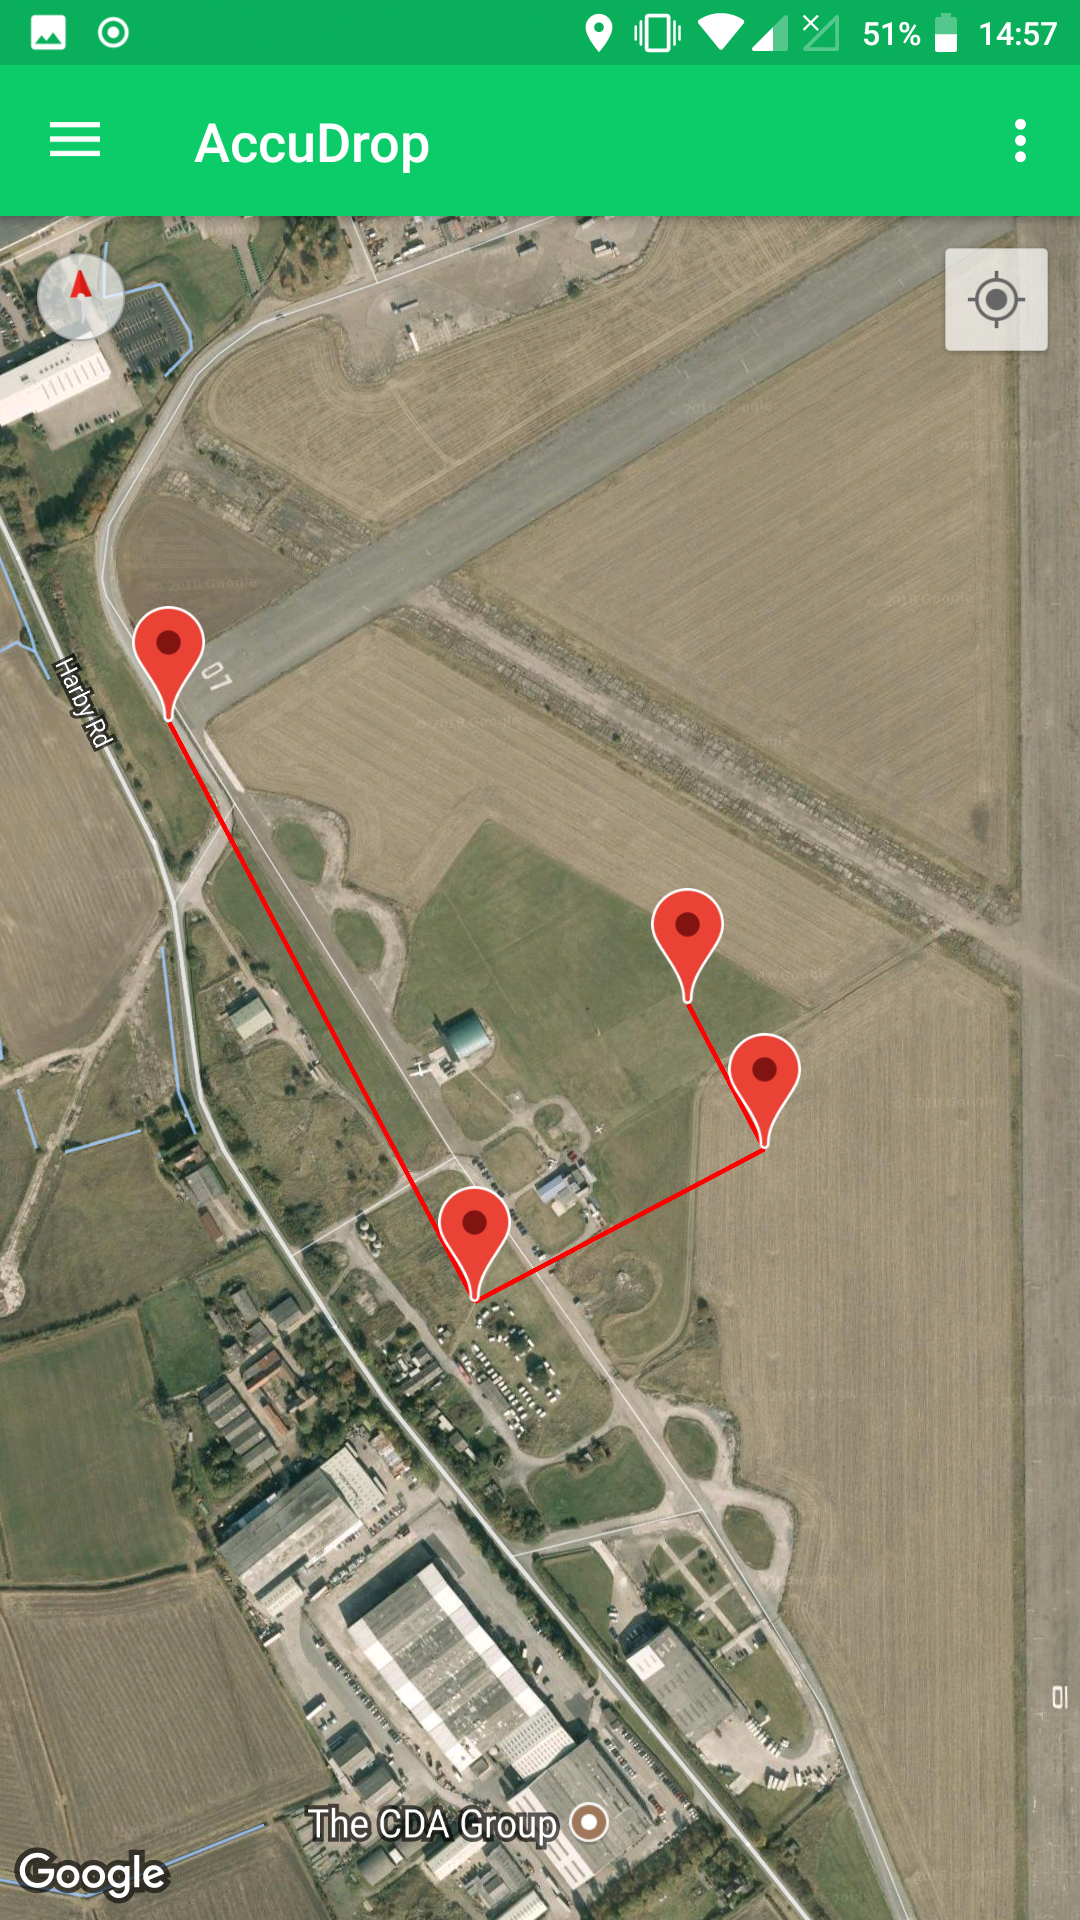
\includegraphics[width=0.45\linewidth]{predicted-landing}
  \hspace{1cm}
  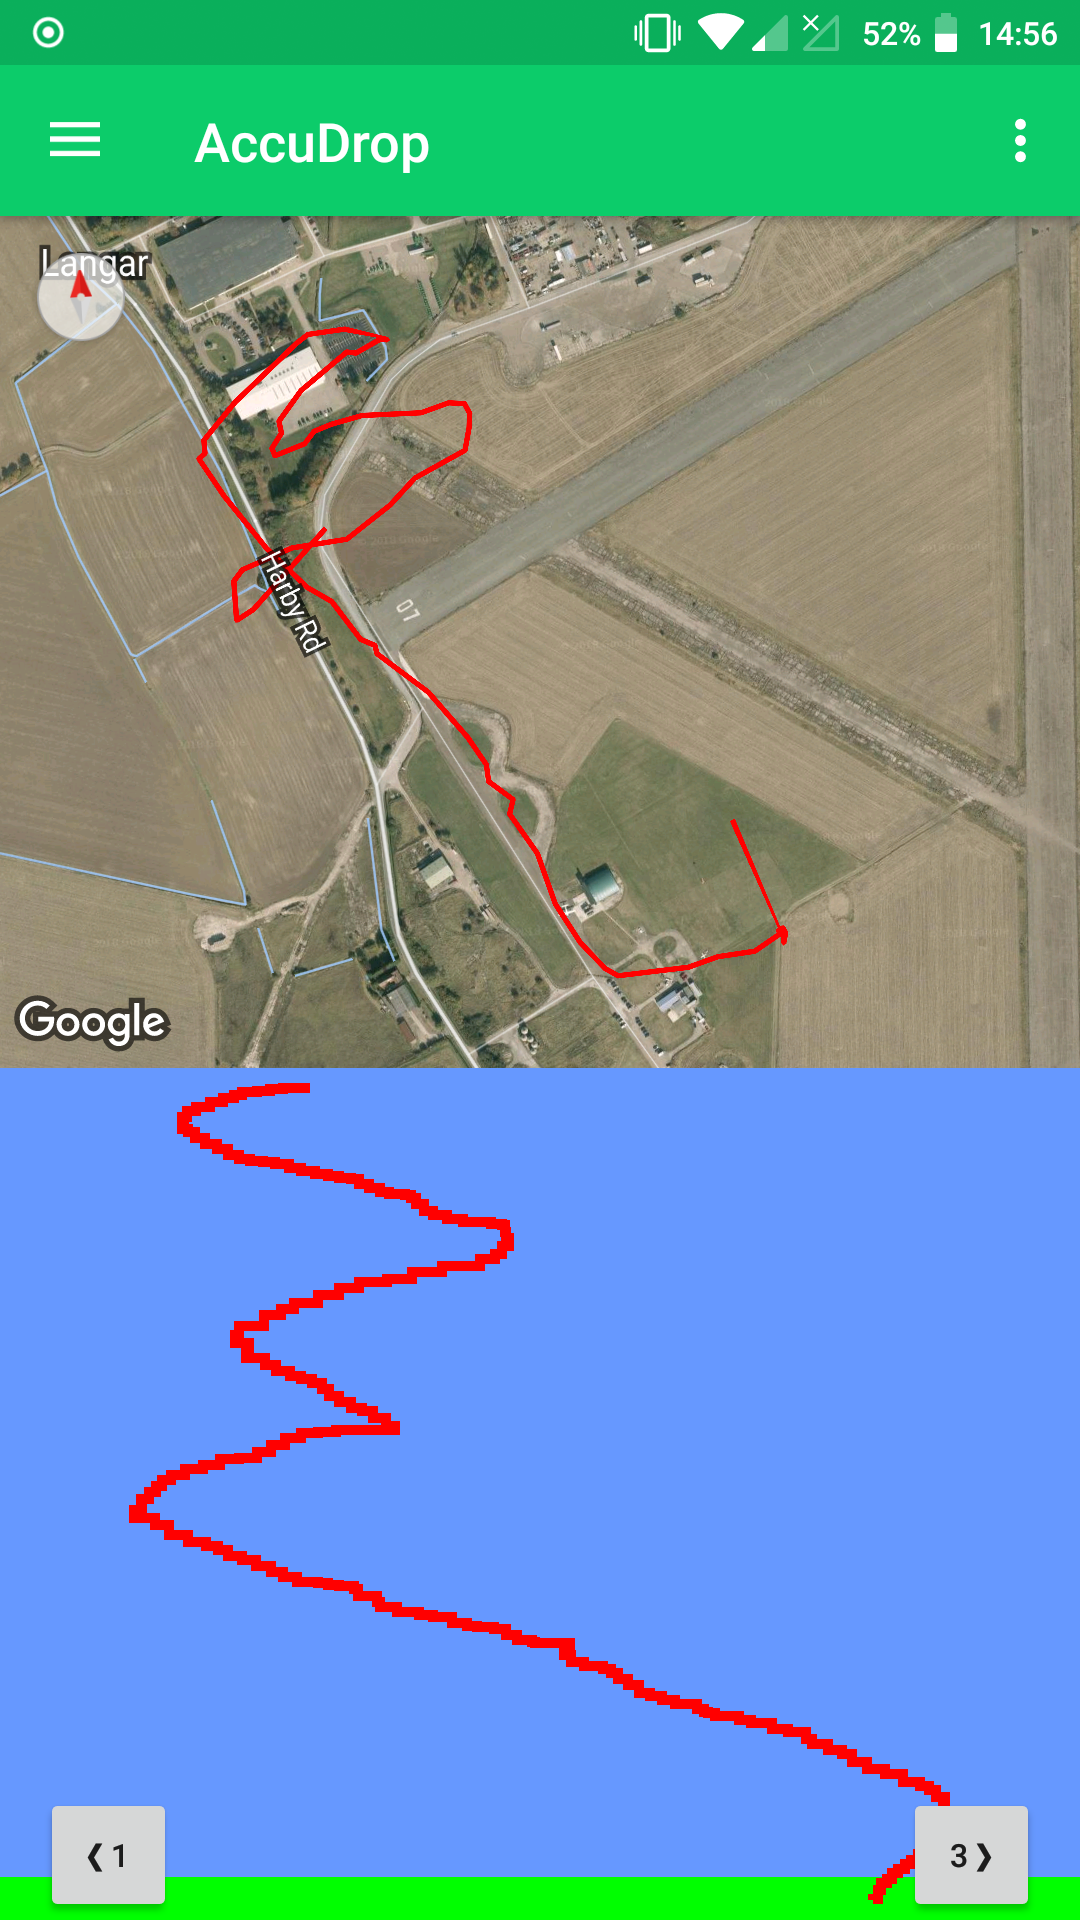
\includegraphics[width=0.45\linewidth]{tracked-landing}
  \caption{A predicted landing pattern (left) and a tracked landing pattern (right) for the same wind conditions and canopy properties. Also shown is the ``holding area'' data before the tracked landing pattern}\label{fig:predicted-tracked}
\end{figure}

\subsection{Skydive Logging}\label{subsec:skydive-logging}
The requirements for the app state that it must be ``able to log the user's jump number, maximum speed and freefall time'' and must be ``able to log the user's landing pattern speed and location''. The app is able to log all of these pieces of data. However, logged speeds are inaccurate due to the method used to calculate them during freefall. Since the altitude data points are so close together (every \SI{300}{\milli\second} in our tests), calculating speed relative to the previous measurement can lead to huge inaccuracies in our computed speed since the time intervals are so small (\SI{\sim300}{\milli\second}) relative to the accuracy of the altimeter readings.

Since skydives were only conducted with the app during the writing of this report, speed calculation was not fixed to produce sane speed results; this meant that speeds could be calculated with an inaccuracy of over \SI{100}{\metre\per\second} during freefall. Inaccuracies also meant that logging prerequisites were met very early in the flight up to altitude. Thus much of the plane journey was tracked in tests.

A feature was added to the app to allow testers to send their database files via email; this meant that we could take a look at the raw data logged by the app during real skydives. Upon receiving the data, we removed much of the positional data from the start of a jump that was the plane journey; this allowed us to then analyse only the jump data. Stopping the skydive logging automatically worked correctly since altitude data was accurate.

\begin{figure}[ht]
  \centering
  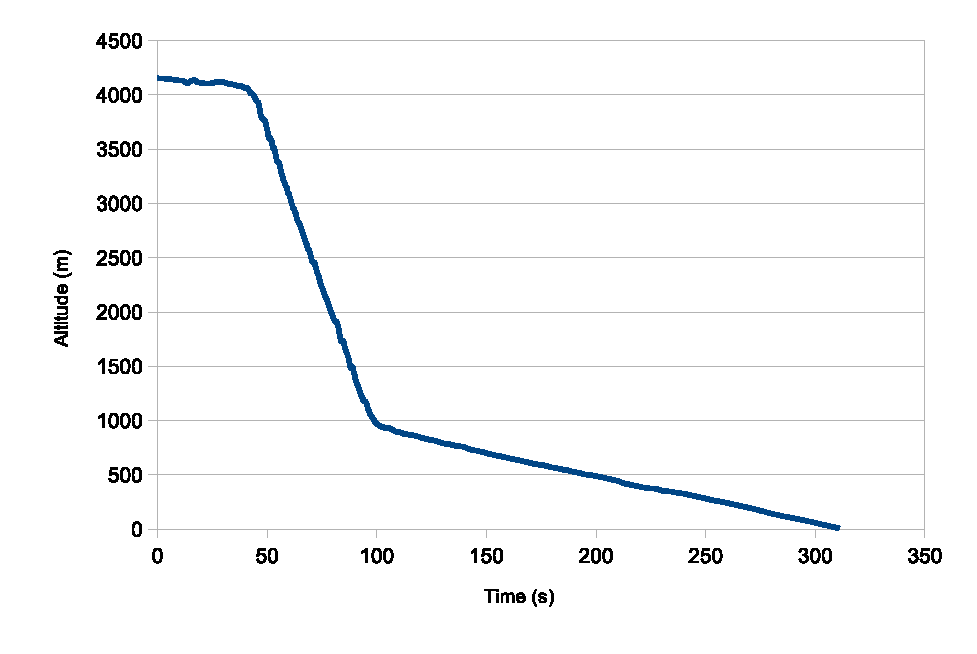
\includegraphics[width=0.8\linewidth]{altitude-time}
  \caption{A graph to show altitude change over time for a skydive logged using the AccuDrop app.}\label{fig:altitude-time}
\end{figure}

Figure~\vref{fig:altitude-time} shows a graph of altitude over time from data exported from a user's database file after a skydive. We can see that there is a smooth line of altitude over time, freefall is visible as the steep drop in altitude and canopy flight can be seen as the shallower descent. According to the data recorded by the app, the skydiver's plane exit altitude was \SI{4152}{\metre}, this was confirmed to be correct by the skydiver, who's regular altimeter had logged an altitude of \SI{4150}{\metre}. It should be noted that the actual skydiving altimeter rounds the altitude to the nearest \SI{10}{\metre}.

The altitude/time data is accurate to a useful degree where we can take a moving average of the data, and do some exponential smoothing to gain smooth speed data that can be considered accurate enough for its use of analysing a jump. After applying these functions to the data in a spreadsheet, we were able to produce what we believe to be reasonably accurate speed statistics. For example, the testing skydiver reported that their altimeter measurement a maximum fall rate of \SI{58}{\metre\per\second} and our smooth data calculated a maximum fall rate of \SI{59}{\metre\per\second}. The smoothed fall rate data can be seen in Figure~\vref{fig:speed-time}.

\begin{figure}[ht]
  \centering
  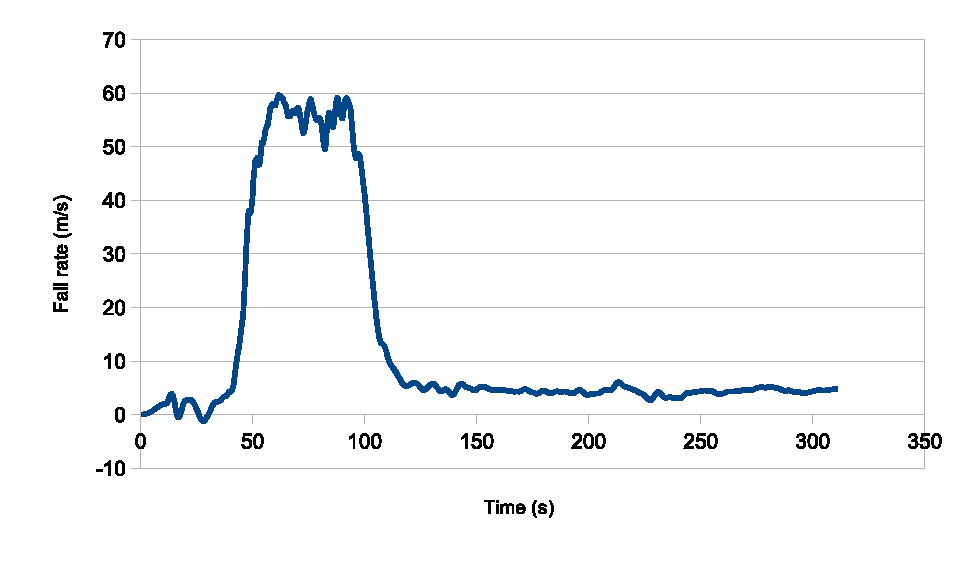
\includegraphics[width=0.8\linewidth]{speed-time}
  \caption{A graph to show fall rate change over time for a skydive logged using the AccuDrop app.}\label{fig:speed-time}
\end{figure}

\subsection{Proximity Warnings}
The requirement that the user should be given warnings of obstacles while under canopy was implemented for the avoidance of other skydivers since skydiver collisions are very dangerous.

The feature was tested by first attempting to connect two devices at the furthest range possible, achieved by having two people walk towards each other until a connection could be made, this was accomplished at a range of \SI{\sim50}{\metre} with a direct line of sight. A warning distance was set for anyone being within a range of \SI{15}{\metre}. The two devices were moved closer to each other until a warning was produced on one phone at a distance of \SI{\sim20}{\metre}, roughly two seconds later, a warning was produced on the second phone.

The proximity warnings are not accurate. However, this would be expected with standard GNSS having an accuracy of \SI{\sim4}{\metre} as mentioned in Section~\ref{subsec:related-work}. It should be noted that the warning in this instance was produced at a longer distance which does raise any safety concerns. The feature should never be relied on entirely over existing safety measures, and so the feature can only increase the safety of a skydiver.

Unfortunately, the feature is limited by the features of Android that require that connections be manually accepted by a user, meaning that if a connection is lost during a skydive then it cannot be made again without user input. This limitation could be overridden by ``rooting'' the phone to allow modifications to the system.

\subsection{Landing Pattern Review}
The landing pattern review screen works as intended and fulfils the user requirement, only displaying the jump positions that have been marked as the canopy fall type.

Figure~\vref{fig:velocity-tracking} shows that the app successfully tracks and displays both the canopy flight in the holding area and the landing pattern after, as expected. We can see using this feature that the GNSS locational data is occasionally slightly incorrect, as occasionally there are some twists in the pattern shown that were not flown.

Since the landing pattern data can successfully be seen in the app, this can be used to come to conclusions on how to improve a landing pattern if applicable.

\subsection{Formation Review}
The formation review feature that was not originally planned but was added to the project during development, could not be tested for a real skydive since we did not have more than one person with a compatible device skydiving at the same time.

Since formation skydiving is done with skydivers in close proximity, we can assume that due to the inaccuracies of GNSS and differences in devices, the data would not be accurate enough for useful comparison of user locations.

Generated data shows that the feature does work and can be useful for reviewing a skydive with others when the positional data is more accurate.

\subsection{Logbook Statistics}
The displaying of skydive logbook statistics works correctly; data is correctly displayed after being queried from the database.

Since actual skydiving data was only collected during the writing of this report, faults in the calculation of fall rates were only realised recently when time could not be dedicated to making alterations to the app. The incorrect fall rate calculations caused jumps to be recorded earlier than they should be and incorrect classification fall type for positional data. The effect of these errors can be seen in Figure~\vref{fig:jump-stats} with the long jump times and extremely fast fall rates.

\begin{figure}[ht]
  \centering
  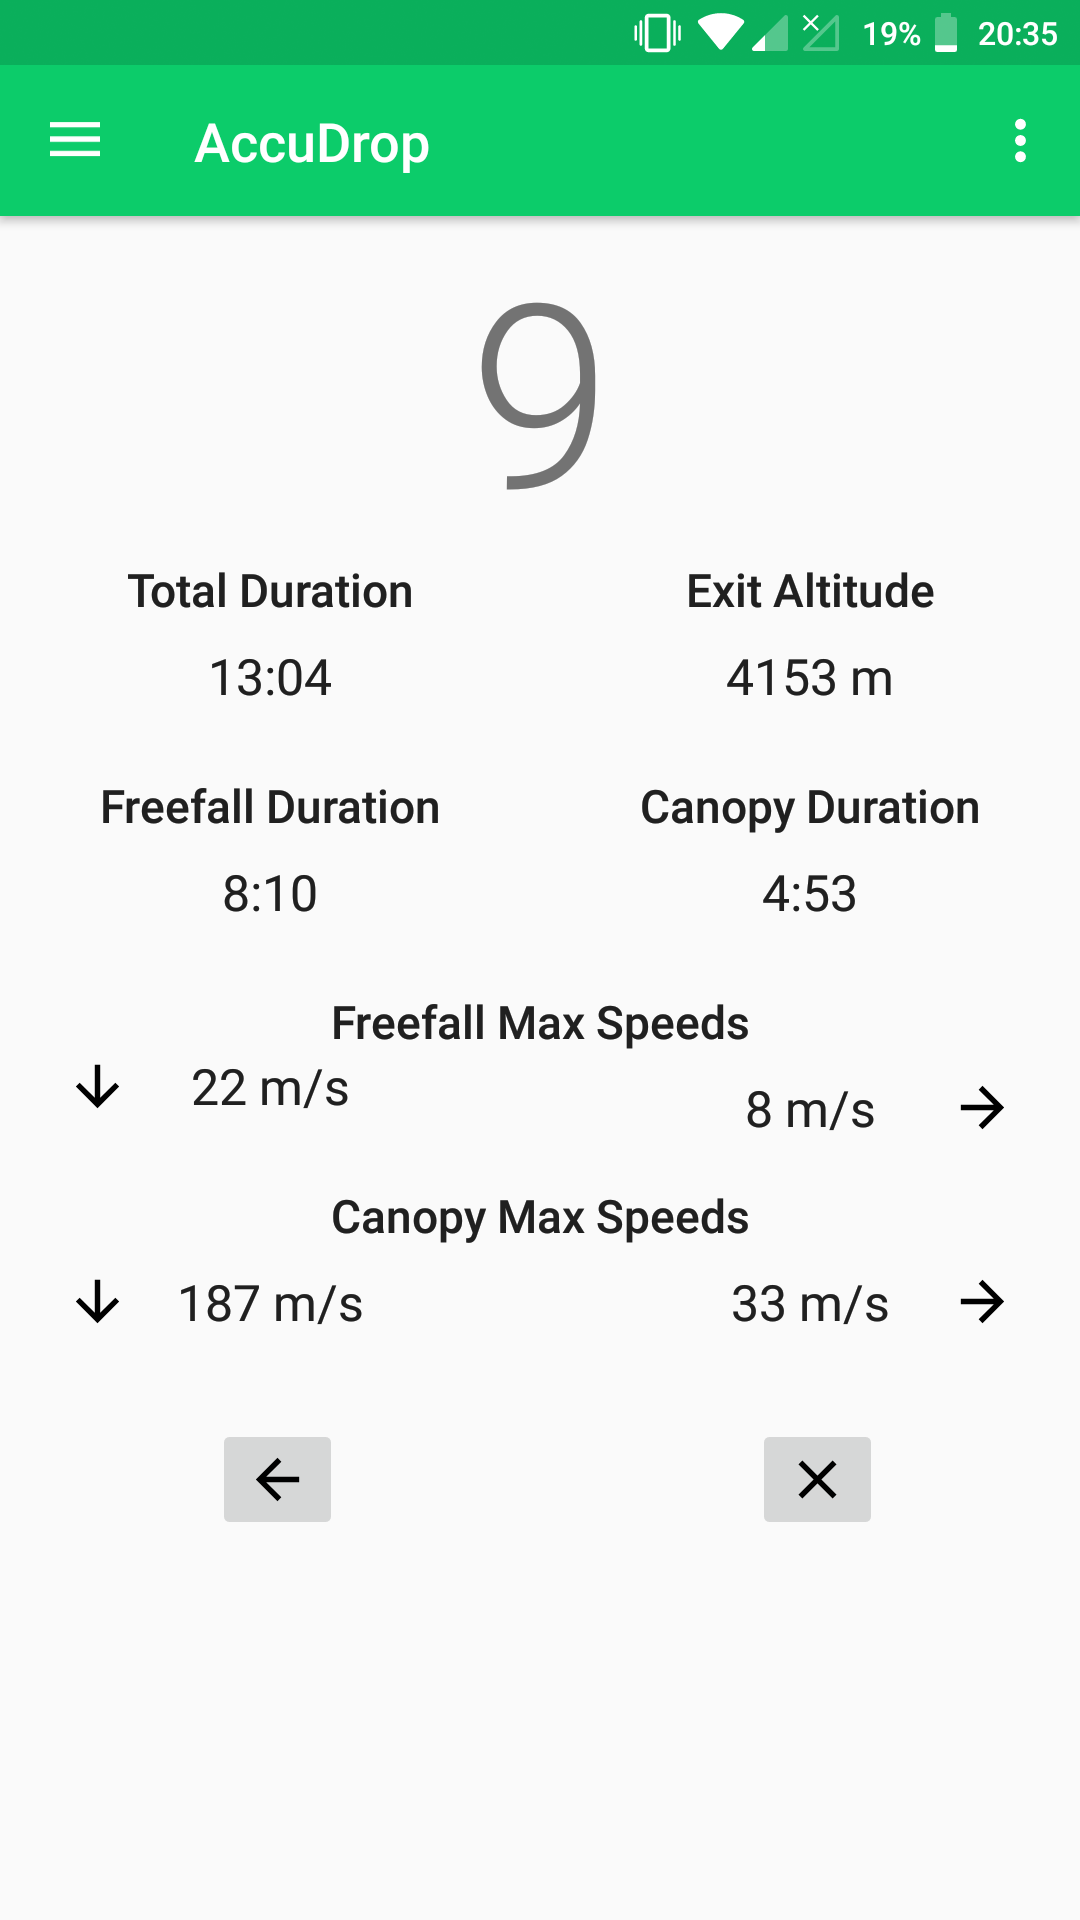
\includegraphics[width=0.3\linewidth]{jump-stats}
  \caption{Incorrect data shown in the logbook statistics feature.}\label{fig:jump-stats}
\end{figure}

As mentioned in Section~\ref{subsec:skydive-logging}, correct fall rates could be calculated with some filtering and averaging of the data, resulting in correct data to show on this screen.

\subsection{User Evaluation}
App testers during the project were asked to give some comments on the app having used it; these are listed below.

\begin{quote}
``The app is easy to set up and forget about during jump, so it does not cause a safety risk by becoming a distraction. The plotting of landing patterns is useful for helping to improve accuracy post jump, and speed calculations (when working) will make it easier to jump with other people as you will be able to compare freefall speeds.''
\end{quote}

\begin{quote}
``The emergence of an app that can be used for improving a skydiver's skills is certainly welcome. I found the landing pattern planning and reviewing features most useful and look forward to what might be accomplished when device communication issues are smoothed out. Hopefully, this app or another app like it can continue development.''
\end{quote}
